\section{ Pakkolaukaisu }
\label{pl-alkeiskoulutuksen-suoritukset-pakkolaukaisu}


Ensimmäiset hyppysi ovat pakkolaukaisuhyppyjä. Irtautuessasi koneesta pakkolaukaisujärjestelmä avaa päävarjon repun ja vetää sisäpussin ulos repusta. 

\subsection{ Oppilaan toiminta }
\label{pl-alkeiskoulutuksen-suoritukset-oppilaan-toiminta}


Uloshyppyasennon tulee olla symmetrinen X-asento tai delta-asento (riippuen konetyypistä), taivutus tulee olla riittävä ja asennon tulee säilyä aina laskuvarjon aukeamiseen saakka. Vapaapudotusta ei ehdi kertyä vielä pakkolaukaisuhypyillä, mutta raajojen ja kehon asennolla on silti vaikutusta hypyn onnistumiseen. 

\subsection{ Ensimmäiseen hyppyysi valmistautuminen }
\label{pl-alkeiskoulutuksen-suoritukset-ensimmaiseen-hyppyysi-valmistautuminen}


Hyppytapahtuma ei suinkaan ala siitä, kun poistutaan koneesta ilmassa. Jotta kaikki sujuisi hyvin, on tärkeää huolehtia myös valmisteluista. Valmistaudu hyppyyn sekä henkisesti että fyysisesti: riittävä yöuni ja ravinto ovat tärkeitä. Väsyneenä tai nälkäisenä keskittyminen on vaikeaa. Ennen hyppäämään kirjoittautumista (pokalistan täyttöä) kootaan kaikki tarvittavat varusteet ja ilmoittaudutaan hyppäämään. Varusteita on hyvä sovittaa päälle, jotta niihin voi tehdä tarvittavat säädöt ajoissa ennen koneelle lähtöä. Suoritusta harjoitellaan joko itsenäisesti tai hyppymestarin kanssa. 


Mikäli mahdollista, seuraa ennen omaa pokaasi toisten hyppääjien ohjailua varjon varassa nähdäksesi ylä- ja pintatuulien vaikutuksen ohjaamiseen ja laskeutumiseen. 


Ennen koneelle menoa hyppymestari tarkastaa, että varusteet on puettu oikein päälle. Tarkastuksen jälkeen varusteita ei saa säätää ilman hyppymestarin lupaa. Vallitsevan tuulen mukainen ohjauskuvio käydään vielä läpi ennen koneelle menoa. Oppilaat saavat mennä koneelle vain hyppymestarin johdolla. 

\subsection{ Oppimistavoitteet }
\label{pl-alkeiskoulutuksen-suoritukset-oppimistavoitteet}


Oppilaan on saavutettava välttämättömät oppimistavoitteet hyväksytysti jotta hyppysuoritus voidaan hyväksyä. 

\begin{enumerate}[label=\bfseries \arabic*)]
\item  Rintamasuunta kohti suhteellista ilmavirtaa uloshypyssä 
\item  Stabiili, symmetrinen uloshyppyasento 
\item  Ajankulun arvioiminen laskemalla (3. hyppy) 
\item  Hyppymestarin tai koneen näkeminen (3. hyppy)  
\end{enumerate}
\subsection{ Hyppylennolla }
\label{pl-alkeiskoulutuksen-suoritukset-hyppylennolla}


Kone kuormataan yleensä käänteisessä järjestyksessä eli se, joka menee koneeseen ensimmäisenä hyppää viimeisenä (poikkeuksena hyppymestari). Varo varusteiden tarttumista koneessa oleviin ulokkeisiin aina koneessa liikkuessasi. Suojaa erityisesti varjojen aukaisukahvoja. Jos takerrut kiinni johonkin, älä revi väkisin vaan ilmoita hyppymestarille. Vältä turhaa liikkumista. Pidä mahdolliset istuinvyöt kiinni, kunnes hyppymestari aukaisee ne tai antaa luvan aukaisuun. Jos lennon aikana huomaat omissa tai muiden varusteissa jotain poikkeavaa, ilmoita siitä heti hyppymestarille. Keskity omaan hyppyysi. Huomioi muut koneessa olijat äläkä häiritse heidän keskittymistään. Koneen päällikkö on lentäjä, mutta sinun päällikkösi on hyppymestari. 

\subsection{ Hypyn kulku }
\label{pl-alkeiskoulutuksen-suoritukset-hypyn-kulku}


Hyppymestari tarkistaa varusteesi ennen koneen oven aukaisua. Lähestyttäessä suunniteltua hyppypaikkaa koneen ovi aukaistaan. 

\begin{description}
\item[101] \hfill \\ 
Otetaan X-asento ja taivutus tai delta ja taivutus (jalat lähes suorina). \hfill \\ 
\end{description}
\begin{description}
\item[102..105] \hfill \\ 
Pidetään taivutus ja asento. \hfill \\ 
Varjo avautuu ja tehdään sen lopullinen avaaminen. \hfill \\ 
\end{description}
\begin{description}
\item[105] \hfill \\ 
Vilkaistaan olkapään yli tarvittaessa. \hfill \\ 
\end{description}

Varjon avauduttua tehdään päätös LENTÄÄ / LENTÄÄ - SELVITÄ / EI LENNÄ ja aloitetaan laskeutumisen suunnittelu. 

\subsection{ Uloshyppy / Cessna 206 }
\label{pl-alkeiskoulutuksen-suoritukset-uloshyppy-cessna-206}


Hyppymestarin komennolla OVELLE! siirrytään (varoen repun osumista koneeseen) ovelle uloshyppyasentoon. Komennolla MENE! ponnistetaan irti koneesta, otetaan hyvä taivutus ja delta-asento sekä aletaan laskea. Rintamasuunnan on pysyttävä koko ajan suoraan koneen lentosuuntaan. Uloshypyssä maa vetää helposti katsetta puoleensa. Jos katsoo maahan eikä koneeseen, taivutus todennäköisesti kääntyy väärinpäin. Ihmisen vartalo kääntyy yleensä katseen suuntaan, joten kun uloshypyn aikana katsoo ylös koneeseen, niin vartalo on taipunut oikeanlaiselle kaarelle. Taivutus lähtee lantiosta (myös selkä ja niska). Tärkeintä uloshypyssä on taivutus. Delta-asennossa kädet ovat n. 45 astetta irti kyljistä, olkapäät takana. Jalat pidetään noin hartioiden levyisessä haara-asennossa ja vain hiukan koukistettuna. Laskeminen on tärkeää opetella heti alusta alkaen, sillä se on käytännössä ainoa tapa säilyttää ajantaju tässä vaiheessa hyppyuraa. Laskeminen tapahtuu ääneen huutamalla (101...105). Uloshyppyharjoituksissa opetellaan oikeaa rytmiä, joten ei huudeta vain numeroita vaan sekunteja. Ilmassa muutama sekunti voi tuntua hyvinkin pitkältä ajalta. 

\subsection{ Uloshyppy / Cessna 182 (streeva) }
\label{pl-alkeiskoulutuksen-suoritukset-uloshyppy-cessna-182-streeva}


Hyppymestarin komennolla OVELLE! siirrytään ovelle. Komennolla MENE! siirrytään (varoen repun osumista koneeseen) roikkumaan streevalle uloshyppyasentoon, irrotetaan ote streevasta ja säilytetään hyvä taivutus sekä X-asento ja aletaan laskea. Rintamasuunnan on pysyttävä koko ajan suoraan koneen lentosuuntaan. Uloshypyssä maa vetää helposti katsetta puoleensa. Jos katsoo maahan eikä koneeseen, taivutus kääntyy todennäköisesti negatiiviseksi. Ihmisen vartalo kääntyy yleensä katseen suuntaan, joten kun uloshypyn aikana katsoo ylös koneeseen, vartalo on taipunut oikeanlaiselle kaarelle. Taivutus lähtee lantiosta (myös selkä ja niska). Tärkeintä uloshyppyasennossa ja uloshypyssä on taivutus. X-asennossa kädet ovat ylhäällä levitettyinä, olkapäät takana. Jalat pidetään noin hartioiden levyisessä haara-asennossa ja vain hiukan koukistettuina. Laskeminen on tärkeää opetella heti alusta alkaen, sillä se on käytännössä ainoa tapa säilyttää ajantaju tässä vaiheessa hyppyuraa. Laskeminen tapahtuu ääneen huutamalla (101...105). Uloshyppyharjoituksissa opetellaan oikeaa rytmiä, joten ei huudeta vain numeroita vaan sekunteja. Ilmassa muutama sekunti voi tuntua hyvinkin pitkältä ajalta. 


\end{multicols}\pagebreak\begin{multicols}{2} 

\section{ Harjoitusveto }
\label{pl-alkeiskoulutuksen-suoritukset-harjoitusveto}


Harjoitusvedon (HV) tavoitteena on oppia suorittamaan itseaukaisu (IA) laskun mukaan siten, että asento ennen aukaisua, aukaisun aikana ja sen jälkeen säilyy stabiilina. 


Harjoitusvetohypyllä varjo avautuu nopeammin kuin itseaukaisuhypyllä pakkolaukaisujärjestelmän takia. Harjoitusveto on kuitenkin ainoa tapa oppia tarvittava liikesarja. Varjon aukeamisesta huolimatta toimenpiteet tehdään aina harjoitellulla tavalla. Harjoitusvetoihin pääsy vaatii kolme stabiilisti hypättyä, hyväksyttyä pakkolaukaisuhyppyä. Lisäksi hypyn aikana on nähtävä joko kone tai hyppymestari. Myös muistikuvan hypystä ja omasta asennosta on oltava selkeä. Koulutuksen sekä maa- ja valjasharjoittelun jälkeen voidaan lähteä hyppäämään harjoitusvetohyppyjä. 

\subsection{ Oppimistavoitteet }
\label{pl-alkeiskoulutuksen-suoritukset-oppimistavoitteet}

\begin{enumerate}[label=\bfseries \arabic*)]
\item  Rintamasuunta kohti suhteellista ilmavirtaa uloshypyssä 
\item  Stabiili, symmetrinen uloshyppyasento 
\item  Kädet liikkuvat symmetrisesti avausliikkeessä 
\item  HV-kahvan vetäminen onnistuu noin 2-4 sekunnin sisällä uloshypystä (selkeä taivutusvaihe ennen vetoa) 
\end{enumerate}
\subsection{ Hyppylennolla }
\label{pl-alkeiskoulutuksen-suoritukset-hyppylennolla}


Varo varusteiden tarttumista koneessa oleviin ulokkeisiin aina koneessa liikkuessasi. Suojaa erityisesti varjojen aukaisukahvoja. Jos takerrut kiinni johonkin, älä revi väkisin vaan ilmoita asiasta hyppymestarille. Vältä turhaa liikkumista. Pidä mahdolliset istuinvyöt kiinni, kunnes hyppymestari aukaisee ne tai antaa luvan aukaisuun. Jos lennon aikana huomaat omissa tai muiden varusteissa jotain poikkeavaa, ilmoita siitä heti hyppymestarille. Keskity omaan hyppyysi. Huomioi muut koneessa olijat äläkä häiritse heidän keskittymistään. Koneen päällikkö on lentäjä, mutta sinun päällikkösi on hyppymestari. 

\subsection{ Hypyn kulku }
\label{pl-alkeiskoulutuksen-suoritukset-hypyn-kulku}


\begin{Figure}\centering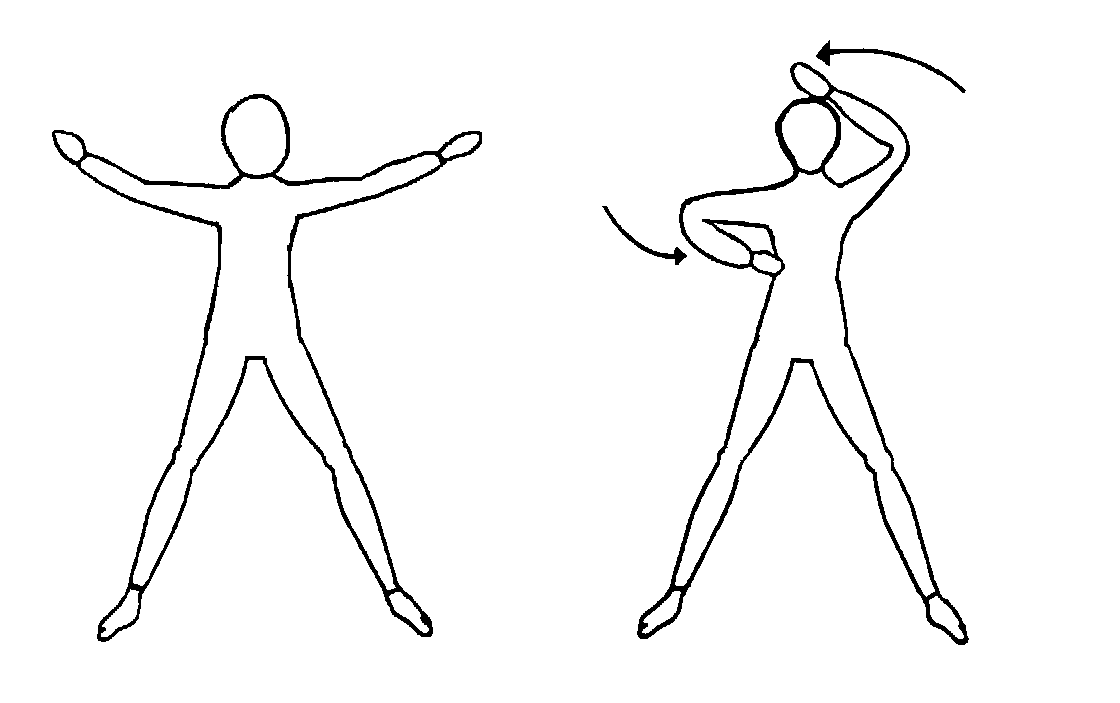
\includegraphics[width=0.7\textwidth]{Harjoitusveto.png}\captionof{figure}{Symmetrinen avausliike}\end{Figure}  

\begin{description}
\item[TAIVUTA (101)] \hfill \\ 
Otetaan X-asento ja taivutus tai delta ja taivutus (jalat lähes suorina). \hfill \\ 
\item[TARTU (102)] \hfill \\ 
vasen käsi kypärän päälle eteen vartalon normaaliksi jatkeeksi ja oikea käsi kahvalle, tiukka ote \hfill \\ 
\item[VEDÄ (103)] \hfill \\ 
veto kahvasta putken tai taskun suuntaan \hfill \\ 
asennon palautus X:ään tai deltaan. \hfill \\ 
\item[101] \hfill \\ 
Aloitetaan laskeminen alusta vedon jälkeen. \hfill \\ 
\end{description}
\begin{description}
\item[102…104] \hfill \\ 
Varjo avautuu ja tehdään sen lopullinen avaaminen. \hfill \\ 
\end{description}
\begin{description}
\item[105] \hfill \\ 
Vilkaistaan olkapään yli tarvittaessa. \hfill \\ 
\end{description}

LENTÄÄ-päätöksen jälkeen laitetaan harjoitusvetokahva pois kädestä (haalarin alle tai rintahihnaan). EI LENNÄ -päätöksen jälkeen pudotetaan harjoitusvetokahva pois ja tehdään varavarjotoimenpiteet. 

\subsection{ Vaaratilanteet }
\label{pl-alkeiskoulutuksen-suoritukset-vaaratilanteet}

\begin{enumerate}[label=\bfseries \arabic*)]
\item  Epästabiili asento: kädet/käsi tai jalat/jalka sisällä --> kaatuu kyljelleen/selälleen --> mahdollista sotkeutua avautuvaan varjoon. 
\item  Veto väärästä kahvasta: päävarjo irtoaa ja varavarjo aukeaa tai varavarjo aukeaa --> varjot voivat sotkeutua toisiinsa. 
\end{enumerate}
\subsection{ Harjoitus }
\label{pl-alkeiskoulutuksen-suoritukset-harjoitus}

\begin{enumerate}[label=\bfseries \arabic*)]
\item  Harjoitellaan suoritusta seuraavasti: 
	\begin{itemize}
	\item  sekunti sekunnilta maassa liikerataharjoituksena 
	\item  sekunti sekunnilta maassa varusteet päällä 
	\item  harjoitusvaljaissa varavarjo- ja vaaratilanteet mukana. 
	\end{itemize}
\item  Annetaan näyte hyppymestarille. 
\end{enumerate}

\end{multicols}\pagebreak\begin{multicols}{2} 

\section{ Itseaukaisu 3'' }
\label{pl-alkeiskoulutuksen-suoritukset-itseaukaisu-3}


Itseaukaisun (IA) tavoitteena on oppia avaamaan laskuvarjo itse. Lisäksi on tunnettava vapaapudotuksen perusteet, osattava poistaa turbulenssi ja osattava pakata itseaukaisuvarjo. Tässä vaiheessa on myös kerrattava varavarjotoimenpiteet ja toiminta apuvarjon yhdyspunoksen tai kantopunoksen kiinnitarttumistilanteissa. 


Itseaukaisuihin pääsy vaatii vähintään kuusi pakkolaukaisuhyppyä, joista kolmella on suoritettu hyväksytty harjoitusveto. Koulutuksen sekä maa- ja valjasharjoittelun jälkeen voidaan lähteä hyppäämään itseaukaisuhyppyjä. Viimeinen harjoitusveto ja ensimmäinen itseaukaisu hypätään samana tai seuraavana kalenterivuorokautena. 


Asennon (X ja taivutus tai delta ja taivutus) ja ajantajun säilyminen sekä korkeuden tarkkailu ovat tärkeitä kaikilla itseaukaisuhypyillä. 

\begin{itemize}
\item  3'' veto 103:lla 
\item  5'' veto 105:llä 
\end{itemize}
\subsection{ Oppimistavoitteet }
\label{pl-alkeiskoulutuksen-suoritukset-oppimistavoitteet}

\begin{enumerate}[label=\bfseries \arabic*)]
\item  Pidä stabiili asento ennen aukaisua ja aukaisun aikana. 
\item  Avaa varjo noin 3 sekunnin sisällä uloshypystä. 
\item  Palauta asento symmetriseksi vedon jälkeen. 
\end{enumerate}
\subsection{ Hyppylennolla }
\label{pl-alkeiskoulutuksen-suoritukset-hyppylennolla}


Varo varusteiden tarttumista koneessa oleviin ulokkeisiin aina koneessa liikkuessasi. Suojaa erityisesti varjojen aukaisukahvoja. Jos takerrut kiinni johonkin, älä revi väkisin vaan ilmoita asiasta hyppymestarille. Vältä turhaa liikkumista. Pidä mahdolliset istuinvyöt kiinni, kunnes hyppymestari aukaisee ne tai antaa luvan aukaisuun. Jos lennon aikana huomaat omissa tai muiden varusteissa jotain poikkeavaa, ilmoita siitä heti hyppymestarille. Keskity omaan hyppyysi. Huomioi muut koneessa olijat äläkä häiritse heidän keskittymistään. Koneen päällikkö on lentäjä, mutta sinun päällikkösi on hyppymestari. 

\subsection{ Hypyn kulku }
\label{pl-alkeiskoulutuksen-suoritukset-hypyn-kulku}

\begin{description}
\item[TAIVUTA (101)] \hfill \\ 
Otetaan X-asento ja taivutus tai delta ja taivutus (jalat lähes suorina). \hfill \\ 
\item[TARTU (102)] \hfill \\ 
vasen käsi kypärän päälle eteen vartalon normaaliksi jatkeeksi ja oikea käsi kahvalle, tiukka ote \hfill \\ 
\item[VEDÄ (103)] \hfill \\ 
veto kahvasta putken tai taskun suuntaan \hfill \\ 
asennon palautus X:ään tai deltaan. \hfill \\ 
\item[101 ] \hfill \\ 
Aloitetaan laskeminen alusta vedon jälkeen. \hfill \\ 
\item[102..104 ] \hfill \\ 
Varjo avautuu ja tehdään sen lopullinen avaaminen. \hfill \\ 
\item[105 ] \hfill \\ 
Vilkaistaan olkapään yli tarvittaessa (turbulenssin poisto). \hfill \\ 
\end{description}

LENTÄÄ-päätöksen jälkeen laitetaan avauskahva pois kädestä (haalarin alle tai rintahihnaan). EI LENNÄ -päätöksen jälkeen pudotetaan avauskahva pois ja tehdään varavarjotoimenpiteet. 


\end{multicols}\pagebreak\begin{multicols}{2} 

\section{ Itseaukaisu 5'' }
\label{pl-alkeiskoulutuksen-suoritukset-itseaukaisu-5}


Tämä on toinen itseaukaisuhyppysi. Irrota streevasta tai ponnista koneesta, laske 101 - 102 - taivuta - tartu - vedä. Kiinnitä edelleen huomiota stabiiliin asentoon, myös vedon jälkeen. Ajantajun on säilyttävä paremmin. 

\subsection{ Oppimistavoitteet }
\label{pl-alkeiskoulutuksen-suoritukset-oppimistavoitteet}

\begin{enumerate}[label=\bfseries \arabic*)]
\item  Pidä stabiili asento ennen aukaisua, aukaisun aikana ja palauta asento symmetriseksi vedon jälkeen. 
\item  Aloita avaustoimenpiteet 4-7 sekunnin sisällä uloshypystä, ja avaa päävarjo. 
\end{enumerate}
\subsection{ Hyppylennolla }
\label{pl-alkeiskoulutuksen-suoritukset-hyppylennolla}

\begin{itemize}
\item Kertaa suoritus mielessäsi 
\item Keskity suoritukseesi 
\item 3X3 -tarkastus ennen hyppyä (\ref{laskuvarjokalusto-ja-hyppyvarusteet-3x3-tarkastus} s.\pageref{laskuvarjokalusto-ja-hyppyvarusteet-3x3-tarkastus}) 
\end{itemize}
\subsection{ Hypyn kulku }
\label{pl-alkeiskoulutuksen-suoritukset-hypyn-kulku}

\begin{description}
\item[TAIVUTA] \hfill \\ 
Tee uloshyppy koneesta ottaen välittömästi ilmavirtaan päästyäsi hyvä taivutus. \hfill \\ 
\item[101] \hfill \\ 
 Säilytä ajantajusi laskemalla.  \hfill \\ 
\item[102 ] \hfill \\ 
Varmistetaan taivutus ja asento. \hfill \\ 
\item[TAIVUTA (103)] \hfill \\ 
Otetaan X-asento ja taivutus tai delta ja taivutus (jalat lähes suorina). \hfill \\ 
\item[TARTU (104)] \hfill \\ 
vasen käsi kypärän päälle eteen vartalon normaaliksi jatkeeksi ja oikea käsi kahvalle, tiukka ote \hfill \\ 
\item[VEDÄ (105)] \hfill \\ 
veto kahvasta putken tai taskun suuntaan \hfill \\ 
asennon palautus X:ään tai deltaan. \hfill \\ 
\item[101 ] \hfill \\ 
Aloitetaan laskeminen alusta vedon jälkeen. \hfill \\ 
\item[102..104 ] \hfill \\ 
Varjo avautuu ja tehdään sen lopullinen avaaminen. \hfill \\ 
\item[105 ] \hfill \\ 
Vilkaistaan olkapään yli tarvittaessa (turbulenssin poisto). \hfill \\ 
\end{description}

LENTÄÄ-päätöksen jälkeen laitetaan avauskahva pois kädestä (haalarin alle tai rintahihnaan). EI LENNÄ -päätöksen jälkeen pudotetaan avauskahva pois ja tehdään varavarjotoimenpiteet. 


\end{multicols}\pagebreak\begin{multicols}{2} 

\section{ 10'' }
\label{pl-alkeiskoulutuksen-suoritukset-10}


Tämä on ensimmäinen hyppysi, jossa vapaapudotusvauhti kasvaa maksimiinsa. Oikea, stabiili ja symmetrinen asento ja hyvä taivutus takaavat hyvän suorituksen. 


Avaustoimenpiteet aloitetaan 1200 metrin korkeudessa mittarin mukaan. Laskemisella säilytetään ajantaju. 

\subsection{ Oppilaan toiminta }
\label{pl-alkeiskoulutuksen-suoritukset-oppilaan-toiminta}

\begin{itemize}
\item Kertaa suoritus mielessäsi 
\item Keskity suoritukseesi 
\item 3X3 -tarkastus ennen hyppyä (\ref{laskuvarjokalusto-ja-hyppyvarusteet-3x3-tarkastus} s.\pageref{laskuvarjokalusto-ja-hyppyvarusteet-3x3-tarkastus}) 
\end{itemize}
\subsection{ Oppimistavoitteet }
\label{pl-alkeiskoulutuksen-suoritukset-oppimistavoitteet}

\begin{enumerate}[label=\bfseries \arabic*)]
\item  Pidä stabiili asento ennen aukaisua, aukaisun aikana ja sen jälkeen.  
\item  Arvioi avauskorkeus mittarin avulla ja aloita avaustoimenpiteet sovitussa korkeudessa. 
\item  Siirry UH-asennosta hypyn aikana perusasentoon. 
\end{enumerate}
\subsection{ Hyppylennolla }
\label{pl-alkeiskoulutuksen-suoritukset-hyppylennolla}

\begin{itemize}
\item Kertaa suoritus mielessäsi 
\item Keskity suoritukseesi 
\item 3X3 -tarkastus ennen hyppyä 
\end{itemize}
\subsection{ Hypyn kulku }
\label{pl-alkeiskoulutuksen-suoritukset-hypyn-kulku}

\begin{description}
\item[TAIVUTA] \hfill \\ 
Tee uloshyppy koneesta ottaen välittömästi ilmavirtaan päästyäsi hyvä taivutus. \hfill \\ 
\item[101..106] \hfill \\ 
 Säilytä ajantajusi laskemalla. \hfill \\ 
 Tarkkaile korkeutta. \hfill \\ 
\item[107] \hfill \\ 
 Vapaapudotusvauhti on maksimissa, rentouta asentoa. \hfill \\ 
\item[1200 metriä] \hfill \\ 
Aloita avaustoimenpiteet. \hfill \\ 
\item[TAIVUTA ] \hfill \\ 
Varmistetaan taivutus ja asento. \hfill \\ 
\item[TARTU] \hfill \\ 
Vasen käsi kypärän päälle eteen vartalon normaaliksi jatkeeksi ja oikea käsi kahvalle, tiukka ote. \hfill \\ 
\item[VEDÄ] \hfill \\ 
Veto kahvasta putken tai taskun suuntaan. \hfill \\ 
Palauta perusasento. \hfill \\ 
\item[101 ] \hfill \\ 
Aloitetaan laskeminen alusta vedon jälkeen. \hfill \\ 
\item[102..104 ] \hfill \\ 
Varjo avautuu ja tehdään sen lopullinen avaaminen. \hfill \\ 
\item[105 ] \hfill \\ 
Vilkaistaan olkapään yli tarvittaessa (turbulenssin poisto). \hfill \\ 
\end{description}

LENTÄÄ-päätöksen jälkeen laitetaan avauskahva pois kädestä (haalarin alle tai rintahihnaan). EI LENNÄ -päätöksen jälkeen pudotetaan avauskahva pois ja tehdään varavarjotoimenpiteet. 

